\documentclass{beamer}

\usetheme[progressbar=frametitle]{metropolis}
%\setbeamertemplate{frame numering}{fraction}
\useinnertheme{metropolis}
\useoutertheme{metropolis}
\usefonttheme{metropolis}
\usecolortheme{spruce}
\setbeamercolor{background canvas}{bg=white}

\usepackage{listings}

\definecolor{codegreen}{rgb}{0,0.6,0}
\definecolor{codegray}{rgb}{0.5,0.5,0.5}
\definecolor{codepurple}{rgb}{0.58,0,0.82}
\definecolor{backcolour}{rgb}{0.95,0.95,0.92}

\lstset{
  basicstyle=\ttfamily,
  keywordstyle=\color{magenta},
  stringstyle=\color{codepurple},
  numbers=left,
  numbersep=5pt,
  numberstyle=\tiny\color{codegray},
  backgroundcolor=\color{backcolour},
  showstringspaces=false,
  tabsize=4
}

\author{Jorge F., Leonidas G., Giordano A.}

\title{Lesson 2}
\subtitle{"Think Big"}

\institute{UTEC}
\date{}

\begin{document}

\begin{frame}
	\titlepage
\end{frame}


\section{Asymptotic analysis}

\begin{frame}{Motivation}

	\begin{itemize}
		\item In 2019, Twitter users send more than 500,000 tweets every minute.
		\item In 2019, 8.1 billion internet users.
		\item In 2018, 2.375 billion monthly active users in Facebook.
	\end{itemize}

	\begin{center}
		This numbers are increasing every day!
		How can services and pages sustain this?
		How can we compare different solutions?
	\end{center}

	\begin{center}
		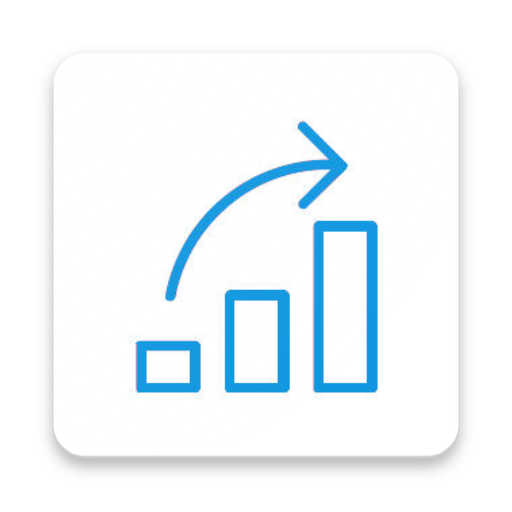
\includegraphics[width=0.23\linewidth]{../img/scalability}

		\textbf{Scalability}
	\end{center}

\end{frame}

\begin{frame}{First Approach: Sampling \& Extrapolation}

	\begin{itemize}
		\item We can measure how long a program takes to run for different input sizes.
		\item This will give us a function we can extrapolate.
		\item Using this method we can experimentally compare different algorithms. 
	\end{itemize}

	\begin{center}
		Is there a better and simpler way to estimate the complexity of algorithms?
	\end{center}
\end{frame}

\begin{frame}{Asymptotic Analysis - Definition}
	A method for defining the mathematical boundaries of the run-time performance or space usage of programs as the input size increases. Useful for estimating the time and space complexity in function of the input size.

	Using the asymptotic analysis we can easily estimate:
	\begin{itemize}
		\item Lower Bound - $\Omega(n)$ Omega notation
		\item Upper Bound - $O(n)$ Big oh notation
		\item \textit{Tight Bound} - $\Theta(n)$ Theta notation
	\end{itemize}
\end{frame}

\begin{frame}{Big O Notation}
	The formal way to express the upper bound of an algorithm running time.
	
	\begin{itemize}
		\item Omit lower terms and coefficients.
		\item $f(n) = O(g(n)) \rightarrow f(n) \leq kg(n)$ for $n > n_0$
	\end{itemize}

	\begin{center}
		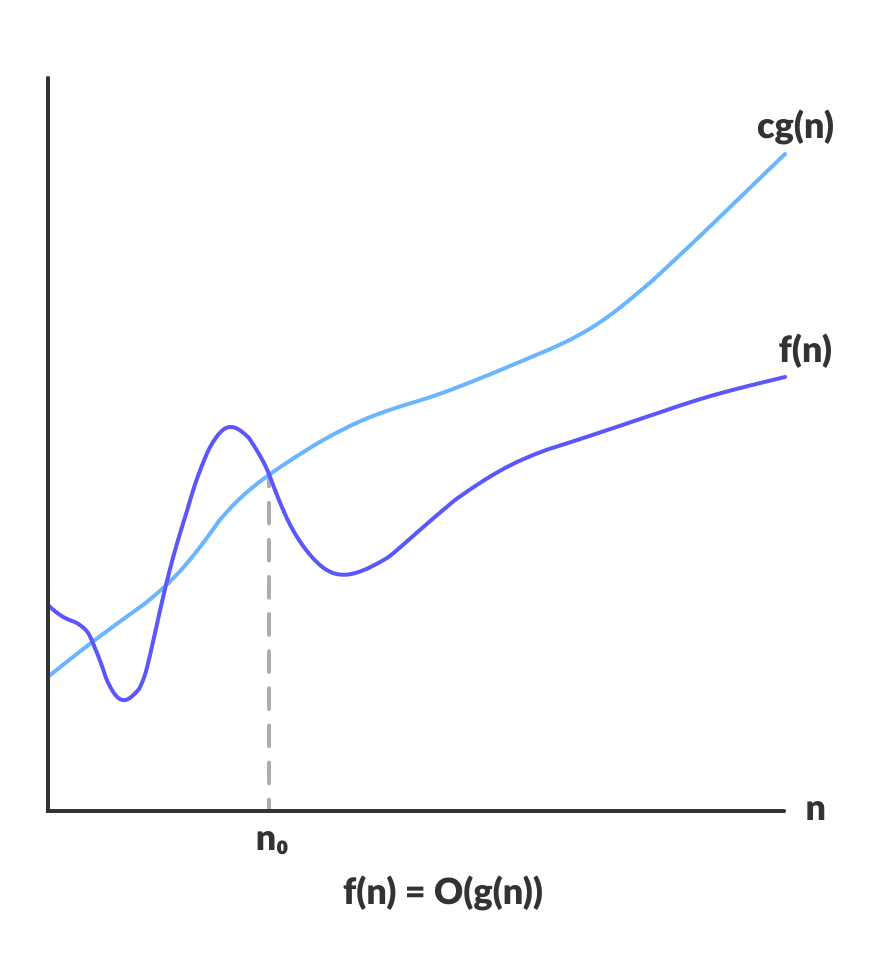
\includegraphics[width=.35\linewidth]{../img/bigO}
	\end{center}
\end{frame}

\begin{frame}{Space Usage vs Running Time}

	There exists almost always a \textbf{trade-off} in an algorithm between space-usage, run-time performance and brain power. Sometimes, we need to save computed values for future actions in order to improve the running time.

	\underline{Example}

	Fibonacci Algorithm

\end{frame}

\begin{frame}{Simplification examples}

	Drop lower terms and multiplicative constants.

	\begin{center}

	$n^3 + n^2 + 1$

	$log(n) + n^2 + 100$

	$0.001*n^3 + 1$

	$ n*log(n) + n^2$

	$ n*log(n) + n + 10^{100}$

	$ n*log(n) + 500*n + 10^{100}$

	$ n*log(n) + n + 2^n$

	\end{center}

	How do we define lower terms? 

\end{frame}

\begin{frame}[fragile]{Examples Linear Algorithm}

\begin{lstlisting}[language=C++]
int main() {
	int ans = 0;
	for (int i = 0; i < 100; i++) {
		if (i % 2 == 0)
			ans += i;
	}
	cout << ans << endl;
	return 0;
}
\end{lstlisting}

\end{frame}

\begin{frame}[fragile]{Examples Quadratic Algorithm}

\begin{lstlisting}[language=C++]
int main(){
	int ans=0;
	for (int i = 0; i < 100; i++){
		for (int j = 0; j < 100; j++) {
			if (i * i == j)
				ans += i;
			if (j - i == i)
				ans -= i;
		}
	}
	cout << ans << endl;
	return 0;
}
\end{lstlisting}

\end{frame}

\begin{frame}{Examples of Time Complexity}
	\begin{center}
		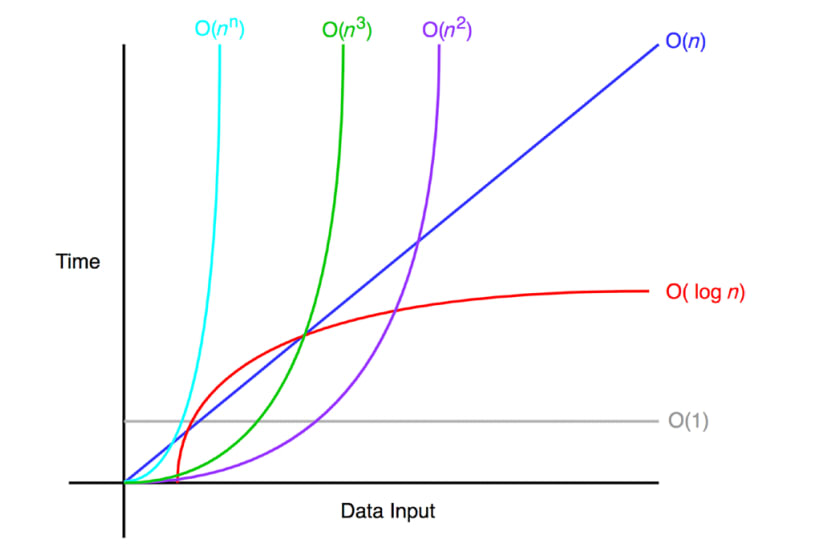
\includegraphics[width=.85\linewidth]{../img/bigOchart}
	\end{center}
\end{frame}

\end{document}
